
%% NE PAS FAIRE DE PRESENTATION PROGRESSIVE !!
%% LE PUBLIC CIBLE NE CONNAIT PAS LES AUTRES METHODES !!!
%% => présenter directement la méthode "idéale"
%% puis, ensuite, dans un supplément facultatif, présenter les alternatives pour mettre en valeur les avantages de IoC.
\section{draft...}


\subsection{Injection de dépendances}
% les beans ne sont plus responsables de trouver leurs dépendances

\begin{frame}[containsverbatim]{Comment gérer autant debriques applicatives ?}
	\framesubtitle{Approche naïve}

	Instanciation des dépendances du bean :
	\begin{lstlisting}
public class EmployeeManager {

  private EmployeeNumberGenerator employeeNumberGenerator;

  private EmailGenerator emailGenerator;

  private EmployeeDAO employeeDAO;

  public EmployeeManager(Datasource datasource) {
    // Generateur de matricule n'a pas de dependance
    employeeNumberGenerator = new EmployeeNumberGenerator();

    employeeDAO = new EmployeeDAO();
    employeeDAO.setDatasource(datasource);// confiruration les datasources !!

    emailGenerator = new EmailGenerator();
    emailGenerator.setEmployeeDAO(employeeDAO); // ajout des dependance
  }
}
	\end{lstlisting}

\end{frame}

\begin{frame}{Comment gérer autant de \emph{briques applicatives} ?}
	\framesubtitle{Approche naïve}

	\begin{alertblock}{Pas de singleton possible}
	Une nouvelle instance d'un bean est créée à chaque fois.
	\end{alertblock}

	\pause
	\begin{alertblock}{Couplage fort}
	La dépendance doit connaitre l'implémentation de ses dépendances, ainsi que les dépendances des dépendances (et ainsi de suite) !
	\end{alertblock}

\end{frame}

\begin{frame}[containsverbatim]{Comment gérer autant de briques applicatives ?}
	\framesubtitle{Approche par \emph{Factory}}

	Utilisation d'une fabrique d'objets
	\begin{lstlisting}
public class EmployeeManager {

  private IEmployeeNumberGenerator employeeNumberGenerator = Factory.getEmployeeNumberGenerator();

  private IEmailGenerator emailGenerator = Factory.getEmailGenerator();
}
	\end{lstlisting}


\end{frame}

\begin{frame}{Comment gérer autant de \emph{briques applicatives} ?}
	\framesubtitle{Approche par \emph{Factory}}

	\begin{exampleblock}{Mutualisation de la création d'objets}
	\begin{itemize}[<+->]
	\item Les méthodes sont réutilisables.
	\item Les implémentations des beans ne sont connues que de la fabrique : utilisation \emph{interfaces}.
	\end{itemize}
	\end{exampleblock}

	\pause
	\begin{alertblock}{Couplage toujours important}
	Dépendance vis à vis de la fabrique.
	\end{alertblock}

	\pause
	\begin{alertblock}{Configuration}
	Comment faire passer la source de données ?
	\begin{itemize}[<+->]
	\item méthode statiquement : peu intuitif et source d'erreurs
	\item argument de la méthode : couplage fort
	\end{itemize}
	\end{alertblock}
% Le code de la fabrique est lourd à écrire...
\end{frame}


\begin{frame}{Comment gérer autant de \emph{briques applicatives} ?}
	\framesubtitle{Approche idéale : injection de dépendances}

	Objectifs de l'approche idéale :
	\begin{itemize}
	\item L'\texttt{EmployeeManager} ne crée pas ses dépendances
	\item Il ne récupère pas ses dépendances d'un tiers
	\end{itemize}

	\pause
	Comment ?
	\begin{itemize}
	\item Il va être créé par un composant externe (équivalent d'une fabrique)
	\item Ce composant externe va lui injecter les dépendances dont il a besoin
	\end{itemize}

\end{frame}


\begin{frame}{Comment gérer autant de \emph{briques applicatives} ?}
	\framesubtitle{Approche idéale : injection de dépendances}

	\begin{block}{Injection de dépendances}
	Le concept d'injection de dépendances est d'instancier un bean, et de lui injecter, par constructeur ou par setter ses dépendances.
	\end{block}
\end{frame}


\subsection{Gestion de la configuration}
% les beans ne sont plus responsables de leur propre configuration

% \begin{frame}{Gestion de la configuration}
% 	\framesubtitle{Approche naïve : accès direct}
%
% 	L'approche de facilité reviendrai à :
% 	\pause
% 	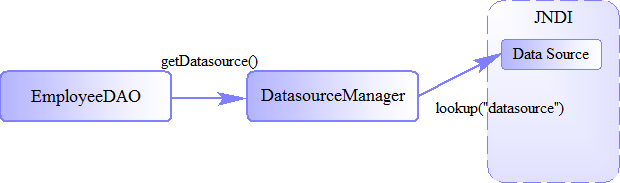
\includegraphics[width=\textwidth]{images/spring_datasource_without.png}
%
% 	\begin{exampleblock}{Exemple}
% 	La couche d'accès aux données utilise un "\texttt{ConnectionManager}" qui récupère les sources de données par \emph{JNDI}.
% 	\end{exampleblock}
%
% \end{frame}
%
% \begin{frame}
%
% 	\begin{alertblock}{Couplage fort}
% 	Aucune flexibilité propre à l'environnement d'exécution n'est permise : les datasources doivent être dans un dictionnaire JNDI dans tous les cas.
% 	\end{alertblock}
% % 	Aucune gestion globale : cohérence des méthodes entre les beans système. Possible duplications de code et impossibilité de partage d'une même configuration.%exemple : nom d'un serveur cible qui risque d'être dupliqué...
%
% 	\pause
% 	Différences sur les environnements :
% 	\begin{itemize}[<+->]
% 	\item Sur un serveur d'application \textbf{OK}.
% 	\item Serveur de test local : nécessite de paramétrer les sources de données
% 	\item En mode standalone (batch) : création d'un "faux" contexte JNDI renseigné à partir d'un autre système de configuration !
% 	\item Tests local (unitaires) : nécessite de forcer la configuration. Ajout de méthodes et lourdeur d'écriture des tests.
% 	\end{itemize}
%
% 	\pause
% 	\begin{alertblock}{Gestion des contextes (portée)}
% 	Si les sources de données dépendent d'un contexte (pays), le DAO doit en être informé.
% 	\end{alertblock}
%
% \end{frame}

\subsection{Cycles de vie}

\subsection{Bilan}

 
